\documentclass[12pt]{article}
\usepackage{polyglossia}
\usepackage{graphicx}
\usepackage{subfig}
\usepackage{amsmath, amssymb, amsfonts}
\usepackage{hyperref}

\usepackage[europeanresistors,americaninductors]{circuitikz}

% Tikz stuff
\usepackage{tikz}

\usetikzlibrary{circuits} % подключаем библиотеки, содержащие
\usetikzlibrary{circuits.ee} % УГО для схем
\usetikzlibrary{circuits.ee.IEC}
\usetikzlibrary{arrows} % подключаем библиотеки со стрелками
\usetikzlibrary{patterns} % и со штриховкой

\usetikzlibrary{%
    decorations.pathreplacing,%
    decorations.pathmorphing%
}

\setdefaultlanguage{russian}
\defaultfontfeatures{Ligatures={TeX},Renderer=Basic}
\setmainfont[Ligatures=TeX]{Times New Roman}
\newfontfamily\cyrillicfont{Times New Roman}[Script=Cyrillic]

\tikzset{circuit declare symbol = ammeter}
\tikzset{set ammeter graphic ={draw,generic circle IEC, minimum size=5mm,info=center:A}}

\tikzset{circuit declare symbol = voltmeter}
\tikzset{set voltmeter graphic ={draw,generic circle IEC, minimum size=5mm,info=center:V}}




\title{Исследование ВАХ лампы накаливания}
\author{Латыпов В.В., Шульга Г.С.}
\date{\today}



\begin{document}

    \maketitle


    \section{Цели и задачи}

    Найти теоретическую форму ВАХ'а лампочки, с помощью методов оптимизации найти коэффициенты в этой зависимости, а затем проверить её на соответствие реальным экспериментальным данным.
    Также можно выяснить, какой вклад вносят теплопроводность и излучение при разных температурах, и в качестве дополнительной задачи выяснить применимость модели абсолютно чёрного тела к исследуемой лампе.

    \section{Теоретические выкладки}
    Для начала рассмотрим лампочку, которая находится в вакууме (стенки её колбы выдерживают разность давлений) и всю электрическую мощность рассеивает в виде светового излучения. Также будем считать, что в данный момент времени лампочка находится в состоянии термодинамического равновесия и её излучение может быть описано приближением абсолютно чёрного тела (АЧТ).

    В соответствии с вышесказанным, применим закон Стефана-Больцмана и запишем условие равенства электрической и световой мощности (светимости):
    \begin{equation}
        \label{1}
        \frac{U^2}{R} = \sigma T^4 S \quad
        \text{,}
    \end{equation}
    где $u$ - напряжение на лампочке в данный момент, $R$ - её статическое сопротивление при температуре $T$,  $S$ - площадь излучающей поверхности.
    Известно,~что~для большинства металлов (в т.ч. - вольфрама) справедлива аппроксимация $ R \propto~ T $ .
    Тогда, если $I$ - ток на лампочке в данный момент, получим:

    \begin{equation}
        \label{2}
        U^2 = \varphi \frac{U^5}{I^5} \quad
        \text{,}
    \end{equation}
    $\varphi$ - коэфф. пропорциональности.

    Окончательно,
    \begin{equation}
        \label{2}
        I = \varphi ^ \frac15  \cdot U ^ \frac35 \propto U ^ \frac35 \quad
    \end{equation}

    В действительности, лампочка отнюдь не находится в вакууме $\Rightarrow$ кроме излучения происходит теплообмен с окружающей средой.
    Таким образом, справедливо уравнение:

    \begin{equation}
        U \cdot I = \alpha \cdot \left( \frac{U}{I} \right) ^ 4 + \beta \cdot \left( \frac{U}{I} \right) + \gamma
    \end{equation}

    Где $\alpha$, ~ $\beta$, ~ $\gamma$ ~ — ~ некие коэффициенты пропорциональности. Свободный член $\gamma$ появляется из-за ненулевой температуры окружающей среды.

    Заменим $U \cdot I$~на~$P$, а $\frac{U}{I}$~ — ~ на $R$:
    \begin{equation}
        \label{approx_formula}
        P = \alpha \cdot R ^ 4 + \beta \cdot R + \gamma
    \end{equation}


    Положим, в ходе эксперимента измерено некоторое количество пар значений напряжения и тока на лампочке.
    Далее, можно произвести следующее инъективное преобразование данных:

    \begin{equation*}
        \label{injection}
        (U, I) \longrightarrow (R, P) = \left( \frac{U}{I}, U \cdot I \right)
    \end{equation*}

    Полученные точки аппроксимируются функцией (\ref{approx_formula}) с помощью классического МНК, и в результате находятся неизвестные коэффициенты $\alpha$,~$\beta$,~$\gamma$~.

    Упомянем ещё один способ нахождения неизвестных коэффициентов в зависимости (\ref{approx_formula}). Рассмотрим следующую аффинную функцию:

    \begin{equation}
        f \left( x, y\right) = \alpha \cdot x + \beta \cdot y + \gamma
    \end{equation}

    График этой функции представляет собой гиперплоскость в $\mathbb{R} ^ 3$ . Заметим, что точки вида
    $ (P, R^4, R) $ принадлежат данной гиперплоскости в соответствии с (\ref{approx_formula}). Однако, т.к. упомянутая формула представляет собой лишь некоторую модель, то в действительности эти точки могут быть лишь аппроксимированы гиперплоскостью с некоторой погрешностью. В итоге, решая уже эту задачу линейной регрессии, можно найти не только оптимальные значения параметров $\alpha$,~$\beta$,~$\gamma$, но и оценить их погрешность.

    \section{Непосредственные измерения}

    Для измерений будем использовать следующую схему:

    {
        \centering
        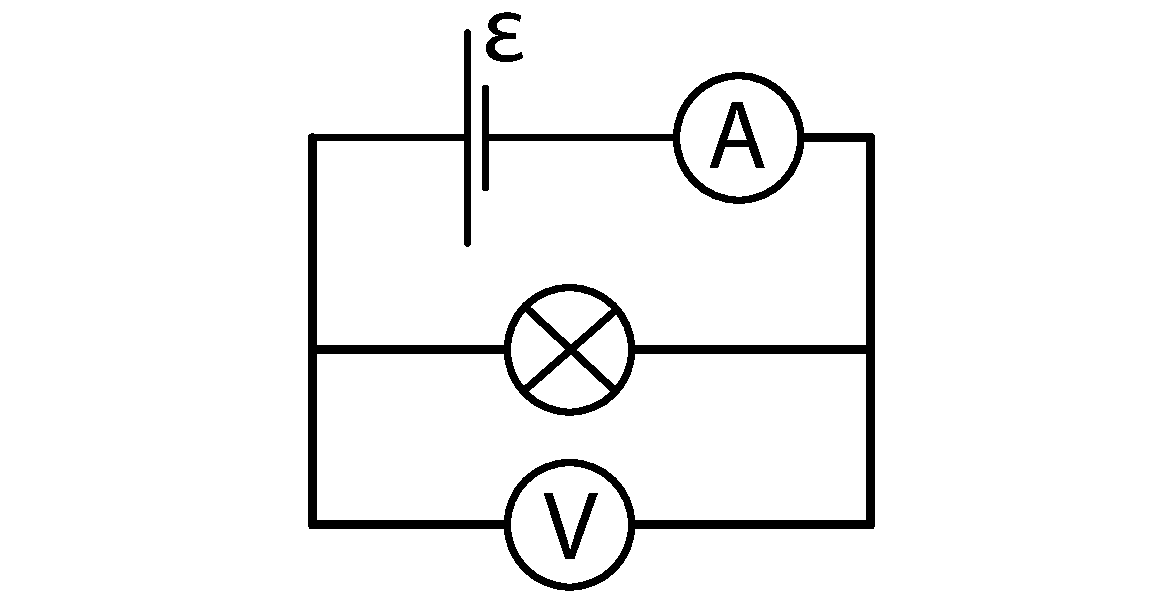
\includegraphics[width=\linewidth]{images/Scheme.pdf}
        \label{fig:scheme}
    }

    {
        \centering
        \begin{tabular}{|l|l|}
            \hline
            Voltage, Volts & Current, Amperes \\ \hline
            0.59    & 0.06    \\ \hline
            0.82    & 0.08    \\ \hline
            0.96    & 0.09    \\ \hline
            1.08    & 0.09    \\ \hline
            1.19    & 0.1     \\ \hline
            1.52    & 0.11    \\ \hline
            1.56    & 0.11    \\ \hline
            1.58    & 0.11    \\ \hline
            1.68    & 0.12    \\ \hline
            1.69    & 0.12    \\ \hline
            1.8     & 0.12    \\ \hline
            2.22    & 0.13    \\ \hline
            2.26    & 0.14    \\ \hline
            2.36    & 0.14    \\ \hline
            2.53    & 0.14    \\ \hline
            2.69    & 0.15    \\ \hline
            2.82    & 0.15    \\ \hline
            2.84    & 0.16    \\ \hline
            2.94    & 0.16    \\ \hline
            3.06    & 0.16    \\ \hline
            3.15    & 0.16    \\ \hline
            3.51    & 0.17    \\ \hline
            3.8     & 0.18    \\ \hline
            4.03    & 0.19    \\ \hline
            4.51    & 0.2     \\ \hline
            5.25    & 0.21    \\ \hline
            6.07    & 0.23    \\ \hline
        \end{tabular}
    }

    \section{Методика обработки измерений}
    В соответствии с теоретическими выкладками, аппроксимируем зависимость $P(R)$ по формуле (\ref{approx_formula}). Получим следующий график:

    {
        \centering
        \includegraphics[width=\linewidth]{images/Resistance_vs_Power_clear_approximation.png}
        \label{fig:resistance_power_approximated}
    }

    Посмотрим на то, какие вклады даёт излучение и теплопроводность при различных значениях напряжения:

    {
        \centering
        \includegraphics{images/resistance_vs_power_with_approximation.png}
        \label{fig:resistance_power_approximated_by_parts}
    }

    Далее, перестроим график $P(R)$ в график вида $U(I)$ по обратному к (\ref{injection}) преобразованию:
    \begin{equation*}
        (P, R) \longrightarrow (I, U) = \left( \sqrt{\frac{P}{R}}, \sqrt{P \cdot R}\right)
    \end{equation*}

    {
        \centering
        \includegraphics[width=\linewidth]{images/Resultant_VAC.png}
        \label{fig:resultant-VAC}
    }
    Оранжевым обозначена модель лампы без учёта теплопроводности (вся электрическая мощность излучается).


    Видно, что рассмотренная модель хорошо описывает эксперимент. Теперь зададимся более сложным вопросом: как вывести закон излучения абсолютно чёрного тела, исследуя ВАХ лампочки? Итак, пусть известен закон Ньютона-Рихмана, а также из общих соображений ясно, что светимость абсолютно чёрного тела $ L \propto~ T^n $ (лампочку будем считать таким телом) Пользуясь N-арным поиском, оптимизируем соответствие (в смысле МНК)~данных~и~новой~аппроксимирующей~функции:
    \begin{equation}
        \label{new_approx_formula}
        P = \alpha \cdot R ^ n + \beta \cdot R + \gamma
        \text{,}
    \end{equation}
    n - параметр поиска.

    {
        \centering
        \includegraphics[width=\linewidth]{images/N-ary_search_dynamic.png}
        \captionof{figure}{зависимость функции ошибки от n}
    }
    Итак, наибольшее соответствие достигается при $n \approx 3.5$, что хорошо согласуется с моделью АЧТ.

    \section{Вывод}

    Рассмотренная модель хорошо описывает эксперимент.
    Более того, мы смогли получить степень зависимости мощности излучения от температуры с приемлемой точностью для весьма неидеальных условий эксперимента. Столь близкое соответствие эмпирической и эталонной степени в зависимости Светимость - Температура может говорить о применимости модели АЧТ к данной лампе накаливания.

\end{document}
